\documentclass[journal=jprobs,manuscript=article]{achemso}

\usepackage[version=3]{mhchem} % Formula subscripts using \ce{}
\usepackage[T1]{fontenc}       % Use modern font encodings
\usepackage{multirow}
\usepackage{subcaption}
\usepackage{booktabs}
\usepackage{hyperref}

\newcommand*\mycommand[1]{\texttt{\emph{#1}}}

\author{Stefan K. Solntsev}
\author{Michael R. Shortreed}
\author{Brian L. Frey}
\author{Lloyd M. Smith}
\email{smith@chem.wisc.edu}
\affiliation[UwMadison]
{University of Wisconsin-Madison}
	
\title[Enhanced Global PTM Discovery (G-PTM-D) with MetaMorpheus]
  {Enhanced Global PTM Discovery (G-PTM-D) with MetaMorpheus}

\begin{document}	

\sloppy

\begin{abstract}

Correct identification of protein post-translational modifications (PTMs) is crucial to understanding many aspects of protein function in biological processes.
G-PTM-D is a recently developed technique for global identification and localization of PTMs.
Spectral file calibration prior to applying G-PTM-D, and algorithmic enhancements in the peptide database search shown here significantly increase the accuracy, speed and scope of PTM identification.
We enhance G-PTM-D by using multi-notch searches, and demonstrate its effectiveness in identification of numerous types of PTMs, including high-mass modifications such as glycosylations.
The changes described in this work lead to a 20\% increase in the number of identified modifications and an order of magnitude decrease in search time.
The complete workflow is implemented in MetaMorpheus, a software tool which integrates the database search procedure, identification of co-isolated peptides, spectral calibration and the enhanced G-PTM-D workflow.
Multi-notch searches are also shown to be useful in contexts other than G-PTM-D, producing superior results when used instead of standard narrow-window and open database searches.
\end{abstract}

\section{Introduction}

Many types of protein post-translational modifications (PTMs) are known, and databases containing detailed information about such modifications are readily available\citep{Creasy_2004}.
Information about a modification often includes the chemical or isotopic composition, mass, specificity to certain residues, and possible restriction of placement to peptide or protein termini.
Protein databases such as UniProt\citep{Uniprot_2017} include information on the localization of specific modifications to specific residues in the protein, but this information is far from complete.
Despite the extensive cataloging of the different protein modifications, their comprehensive discovery and identification in complex biological samples has continued to pose a challenge for proteomics\citep{Olsen_2013}.

Numerous procedures for identification and localization of PTMs from "bottom-up" tandem mass spectrometric datasets exist.
These primarily address common modifications (e.g. phosphorylations) in well-studied systems, but global discovery tools, such as MODa\citep{Na_2011} and G-PTM-D\citep{Li_2016}, for identification and localization of a wide variety of different PTMs are also available.
G-PTM-D was developed in our laboratory and consists of three stages: 1) A wide precursor mass tolerance database search ('open' search)\citep{Chick_2015, Na_2011}, which provides mass differences between the identified peptides and the observed precursor peptide masses, hypothesized to differ in mass due to the presence of a PTM;
2) For those peptides for which the mass difference corresponds to the mass of a known PTM, a database augmentation step adds plausible localized PTMs to the corresponding protein entries in the search database;
3) A final standard tight precursor tolerance search ('narrow-window' search) using the augmented database to identify both modified and unmodified peptides subject to a standard false discovery rate (FDR) threshold based upon the target:decoy strategy\citep{Elias_2007}.

While G-PTM-D delivers confident identification of numerous types of PTMs, it has a few significant limitations.
The initial open search is slow, taking hours for modest size datasets.
Thus, high mass modifications such as glycosylations are out of reach, since widening the search window from the suggested $\pm 200$ Da increases the already-slow search time.
The final narrow-window search is also problematic, as it does not account for peptide-spectral matches (PSMs) with mass differences arising from misassignment of the monoisotopic peak during precursor deisotoping.
Discovery of modifications is limited to PTMs in the UniProt database: this is a significant limitation since that database does not include modifications arising from sample handling, and ignoring those modifications significantly degrades the final PTM identification rates.
Finally, PTMs that are similar in mass, such as phosphorylation (79.9663 Da) and sulfonation (79.9568 Da), are problematic since they are virtually indistinguishable in unprocessed spectral files.
These limitations motivated the work described here.

The enhanced G-PTM-D workflow is presented in Figure~\ref{fgr:diagram}.
Spectral calibration is essential for distinguishing modifications with similar mass, and so we recommend running the G-PTM-D procedure on calibrated spectra files: for this purpose we implemented a calibration procedure in MetaMorpheus.
To address the long search times of the open search, we replace the search in the first stage by a specialized search called a multi-notch search that only allows specific mass differences which correspond to pre-selected masses (e.g. PTMs and amino acids).
This change improves the specificity of the search and significantly decreases search time.
The database augmentation step is similar to the original G-PTM-D procedure, but the modification list is significantly expanded to accommodate modifications such as chemical adducts, glycosylations, lipids, and other important modifications.
The final narrow-window search is also replaced by a limited multi-notch search that accommodates errors in the precursor mass deisotoping (+1.0029 and +2.0054), and the capability for identifying co-isolated peptides, further increasing the number of confidently identified peptides and PTMs.

\begin{figure}[H]
  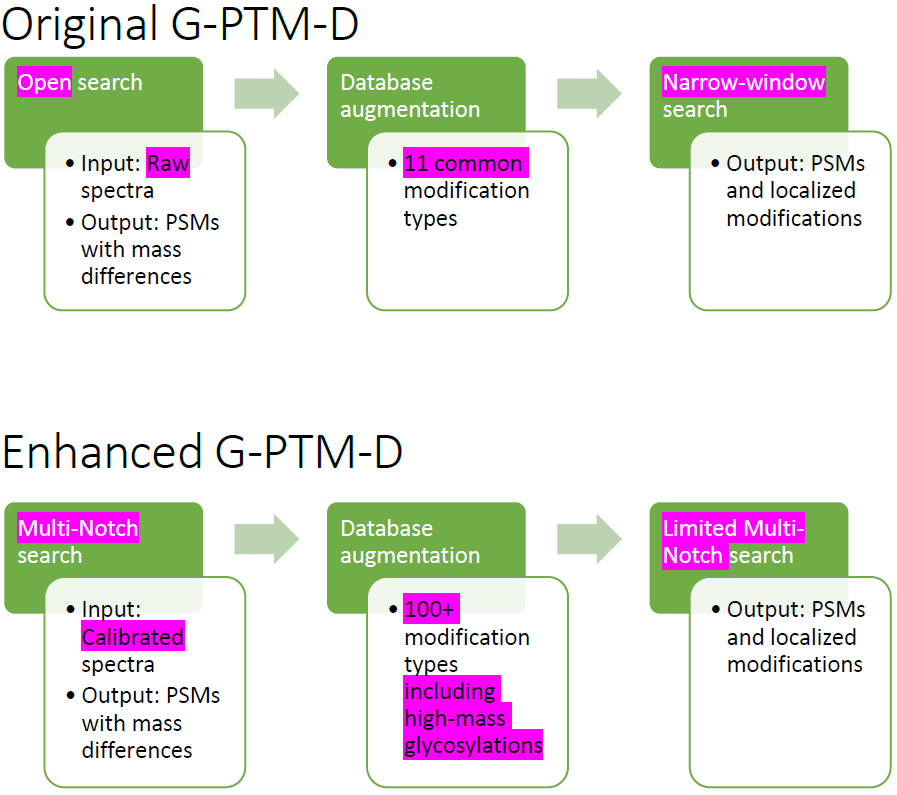
\includegraphics[scale=0.5]{paperDiagram.png}
  \caption{The three steps of the G-PTM-D workflow are indicated in the light beige color. The dark orange color corresponds to the inputs.}
  \label{fgr:diagram}
\end{figure}


\section{Experimental Procedures}

We developed a modified version of the Morpheus software for bottom-up spectral database searching\citep{Wenger_2013} that we call MetaMorpheus, which integrates the database search procedure with spectral calibration and the enhanced G-PTM-D workflow.
MetaMorpheus is freely available at \url{https://github.com/smith-chem-wisc/MetaMorpheus}.
MetaMorpheus heavily utilizes an auxiliary library called mzLib, which is a vast library of software tools for analyzing and processing mass spectral data.
mzLib can be found at \url{https://github.com/smith-chem-wisc/mzLib}.

Three multi-fraction mammalian datasets with deep proteome coverage were used to evaluate performance.
These tryptically digested cell lysates correspond to 28 fractions from human Jurkat cells and 9 fractions from each of two different pancreatic islets from two species of mice.
These datasets are available at \url{https://db.systemsbiology.net/sbeams/cgi/PeptideAtlas/PASS_View?identifier=PASS00215} and \url{https://db.systemsbiology.net/sbeams/cgi/PeptideAtlas/PASS_View?identifier=PASS00470}, and are described in detail elsewhere~\citep{Sheynkman2013, Shortreed_2015, Cesnik_2016}.

UniProt XML protein databases used were downloaded on Sept 14, 2017, and contain only reviewed human/mouse/contaminant proteins.

The database augmentation step allowed 209 modification types, including PTMs, adducts, and chemical modifications. See Supplementary Table 1 for a complete listing.

\section{Results and Discussion}

This work presents four major changes to the previously published G-PTM-D workflow:
a spectral calibration;
a replacement of the open search with a custom multi-notch search for PTM discovery;
replacement of the final traditional narrow-window search with a limited multi-notch search that permits exact matches even when incorrectly deisotoped precursor masses are present;
and lastly, addition of capacity for identification of multiple co-fragmented peptides from a single MS/MS scan.
To clarify the advantage of each change, they are first discussed separately, followed by an analysis of their combined effect upon overall G-PTM-D performance.

\subsection{Calibration}

A critical parameter for peptide identification is mass accuracy\citep{Scherl_2008}.
Higher mass accuracy provides increased specificity and thus confidence in peptide identifications, decreasing the false discovery rate.
Instrument noise, systematic drift and miscalibration all limit the mass accuracy in acquired spectra.
Multiple calibration strategies to improve mass accuracy have been devised and fall into three general categories: external calibration prior to the MS experiment (e.g. standard instrument calibration protocols); internal calibration during the MS experiment (e.g. real-time calibration using a lock mass standard\citep{Olsen_2005}); and spectral calibration subsequent to the MS experiment (post-acquisition spectral calibration).
We developed a post-acquisition calibration procedure that builds upon the software lock mass concept\citep{Cox_2011} recently reported by the Mann group.
In our strategy, the m/z differences between expected and observed peaks in the peptide tandem MS spectra are compiled, and then used to recalibrate the spectra.
The spectral calibration procedure consists of two steps: Step 1: A narrow tolerance (e.g. 10 ppm precursor, 20 ppm fragment) database search is performed on the dataset.
This yields a set of peptide identifications subject to a desired FDR.
Step 2: The identifications from Step 1 provide a theoretical list of m/z peaks that should match closely to observed m/z peaks in the spectra file, and the discrepancies between the theoretical and observed peaks are used to inform a peak shifting procedure.
The calibration algorithm is described in detail in Supplementary Material 2.

We demonstrate the effectiveness of the calibration approach using Jurkat fraction 16 as an example.
Figure~\ref{fgr:fig1-calibErrors} displays the errors in m/z values of MS1 peaks identified by Step 1 of the calibration, both before and after the calibration procedure is applied.
These errors are plotted versus two important variables: the m/z value of the peak and the retention time of the corresponding scan.
In addition to these two parameters, the calibration function native to MetaMorpheus also considers peak intensity, injection time, total ion count, and other variables as potentially influencing the m/z errors.
Calibration successfully removes both linear and non-linear dependencies between the m/z errors and these variables.
Prior to calibration, 95\% of the errors fell between -8.4 and 3.1 ppm, and after calibration 95\% of the errors fell between -1.7 and 2.0 ppm.
MetaMorpheus calibrates both MS1 and MS2 scans (using MS2 fragment matches), but only the results from MS1 are shown here.
MetaMorpheus calibrated files are verified to be compatible with a variety of tools and workflows, including TPP\citep{Deutsch2010}, and MSFragger\citep{Kong_2017}.
In addition to calibrated spectra files, the calibration procedure outputs the standard deviations and averages of the errors post-calibration, which could then be used as search parameters; this is an alternative to using dedicated tools such as Param-Medic\citep{May2017} for determining the best search parameters for a given spectra file.

\begin{figure}[H]
 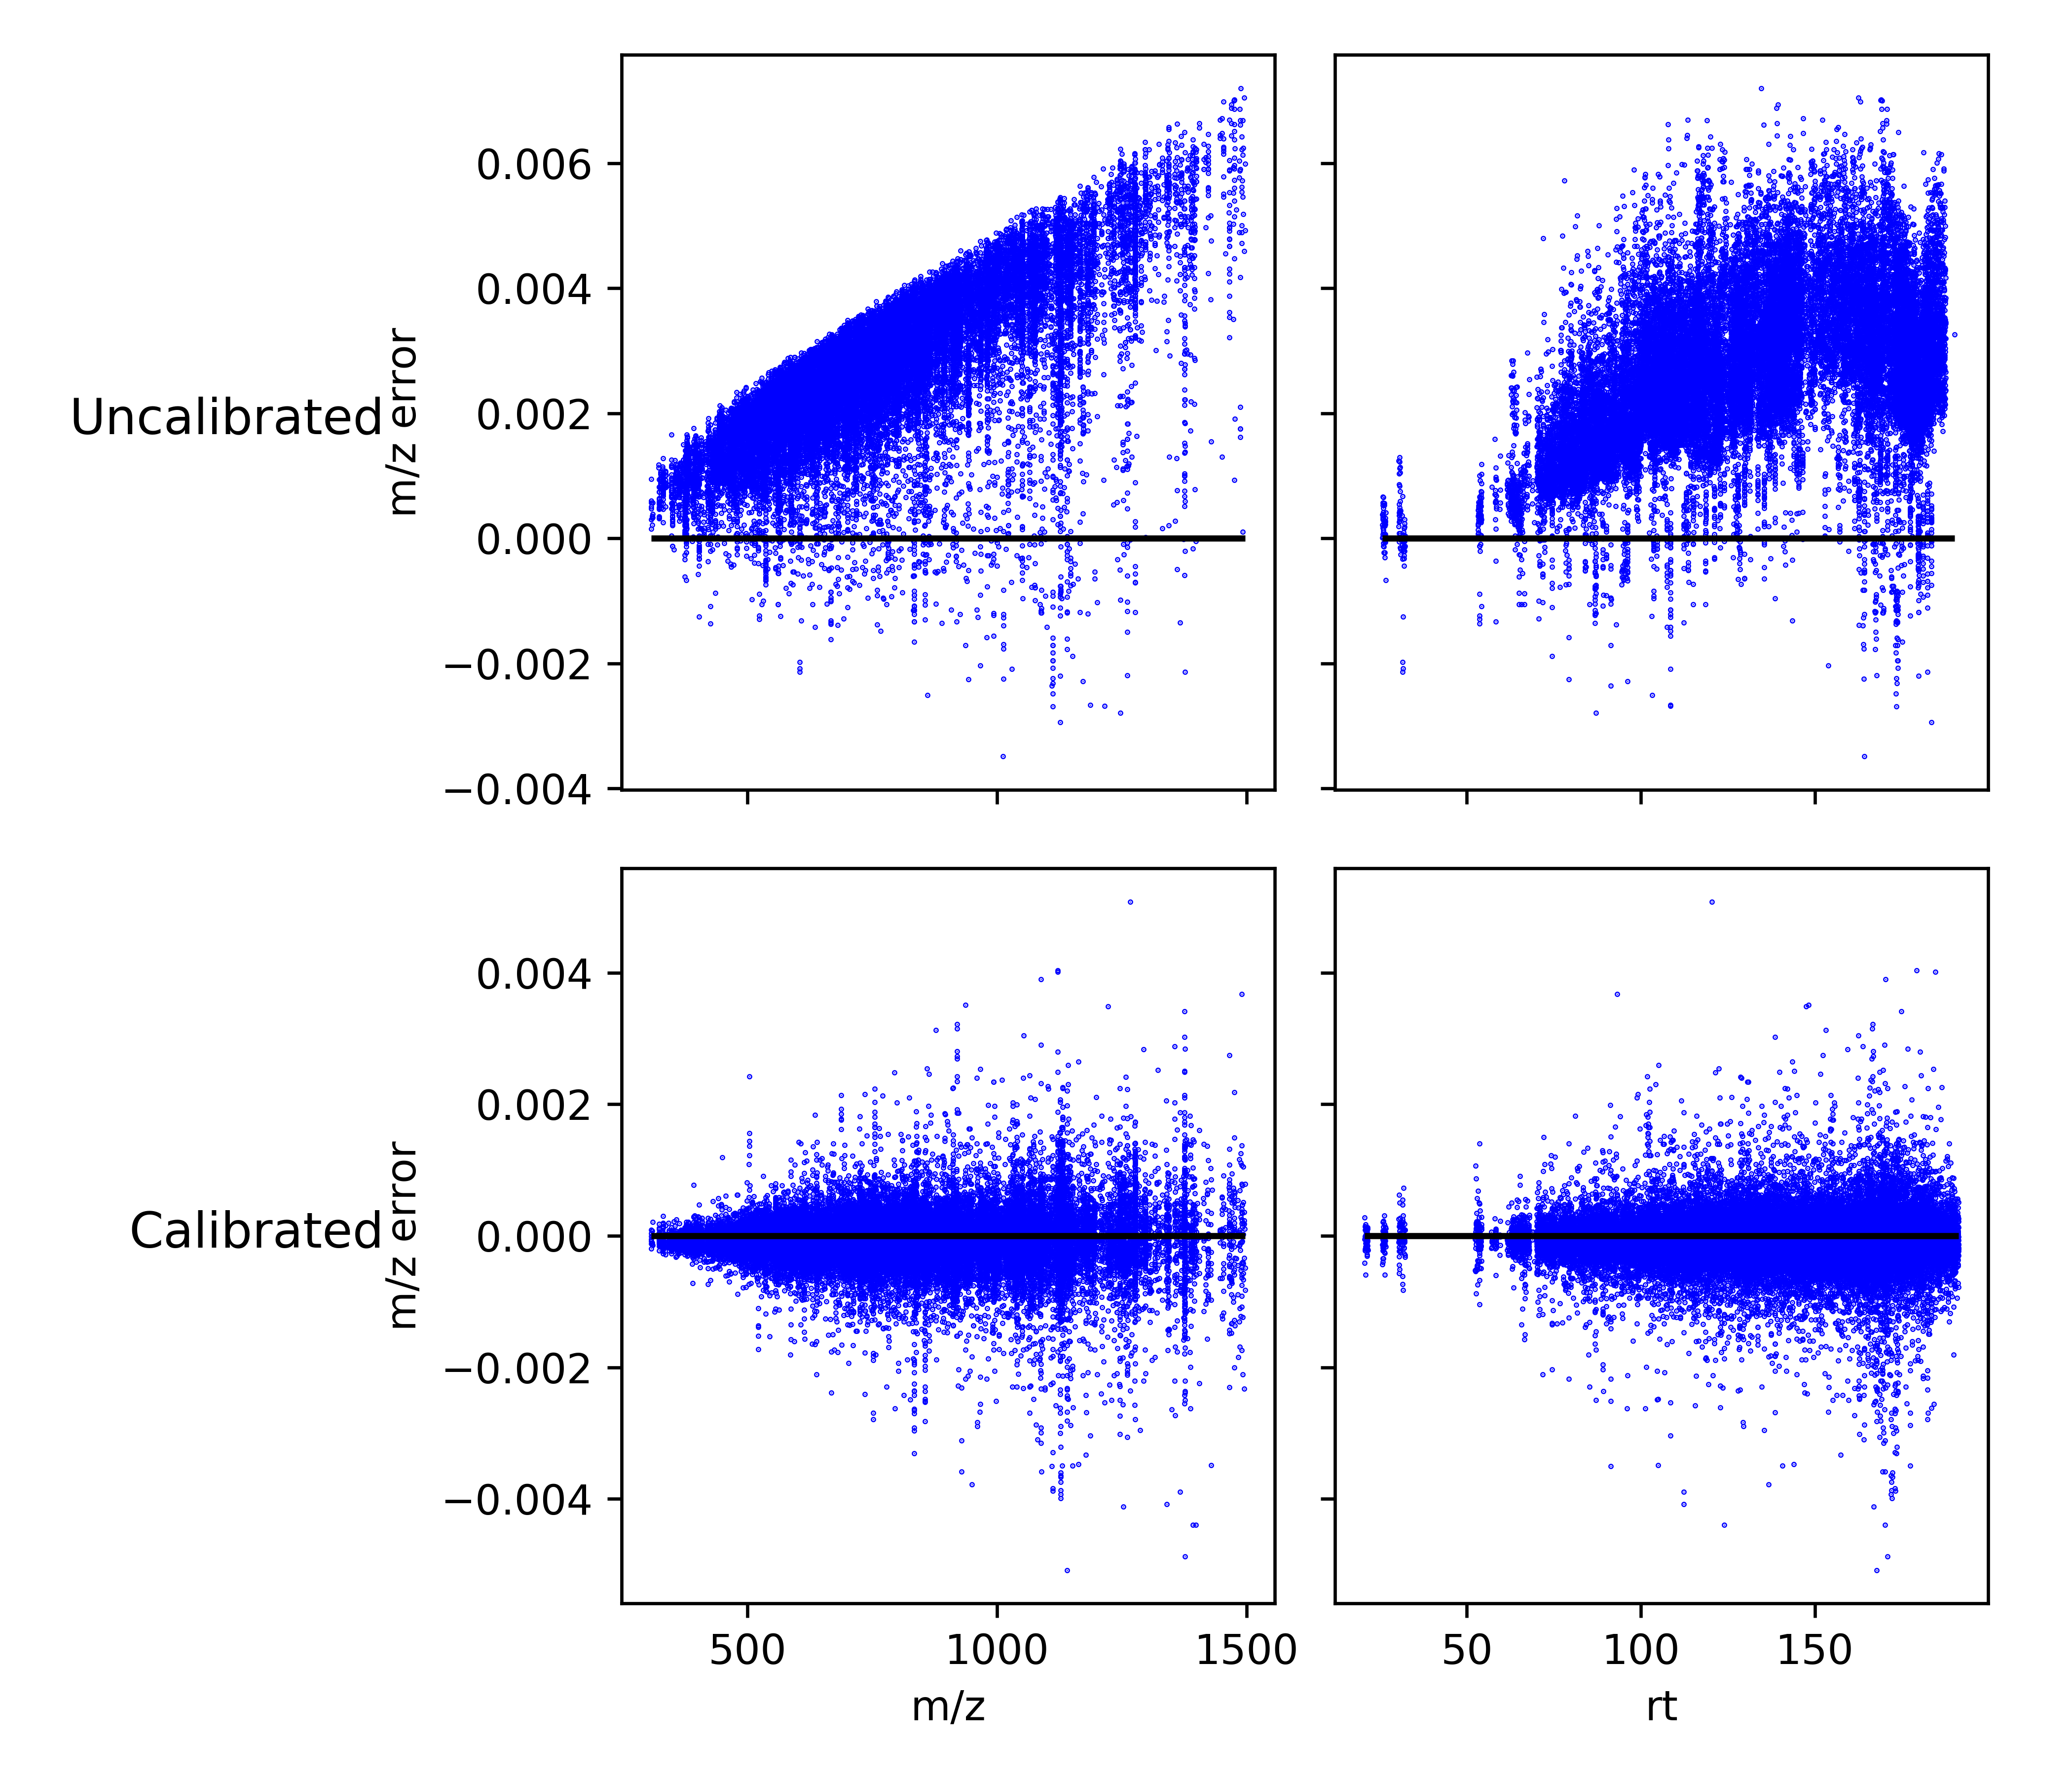
\includegraphics{fig1-calibErrors.png}
 \caption{Errors in m/z value of select peaks before (top panels) and after (bottom panels) calibration. These errors are plotted vs two variables: m/z value (left) and the retention time (right).}
 \label{fgr:fig1-calibErrors}
\end{figure}

Calibration quality improvements are also shown by the results of a standard database search, conducted on uncalibrated versus calibrated spectra using a 10 ppm precursor mass tolerance.
Table~\ref{tbl:calib} details the results of these searches.
The calibration procedure successfully addresses instrument miscalibration by centering the mass errors around zero ppm (-2.08 ppm vs -0.10 ppm).
The systematic noise introduced by various other factors has also been corrected, as evidenced by the decrease in the standard deviation of the errors in the precursor masses, which shows that the calibrated mass spectra predominantly have sub-ppm mass errors.
A beneficial side effect of calibration is a corresponding increase of about 1\% in the number of confidently identified PSMs , when using the same 10 ppm precursor mass tolerance.
Histograms of the mass errors in identified peptides before and after calibration are plotted in Figure~\ref{fgr:fig2-10ppmSearchCalib}.
In summary, the main results of calibration are: more PSMs at 1\% FDR, decreased error in precursor mass, and decreased standard deviation in average mass error.

\begin{table}[]
\centering
\caption{PSMs Within 1\% FDR Before and After Calibration}
\label{tbl:calib}
\begin{tabular}{lll}

                                                                                      & Orig        & Calib        \\
 PSM Count                                                           &      270548   &   273825        \\
 Average Error (ppm)                                                              &      -2.08      &        -0.10      \\
 St. Dev of Error                                                    &       2.24      &        1.06      \\
\end{tabular}
\end{table}

\begin{figure}[H]
 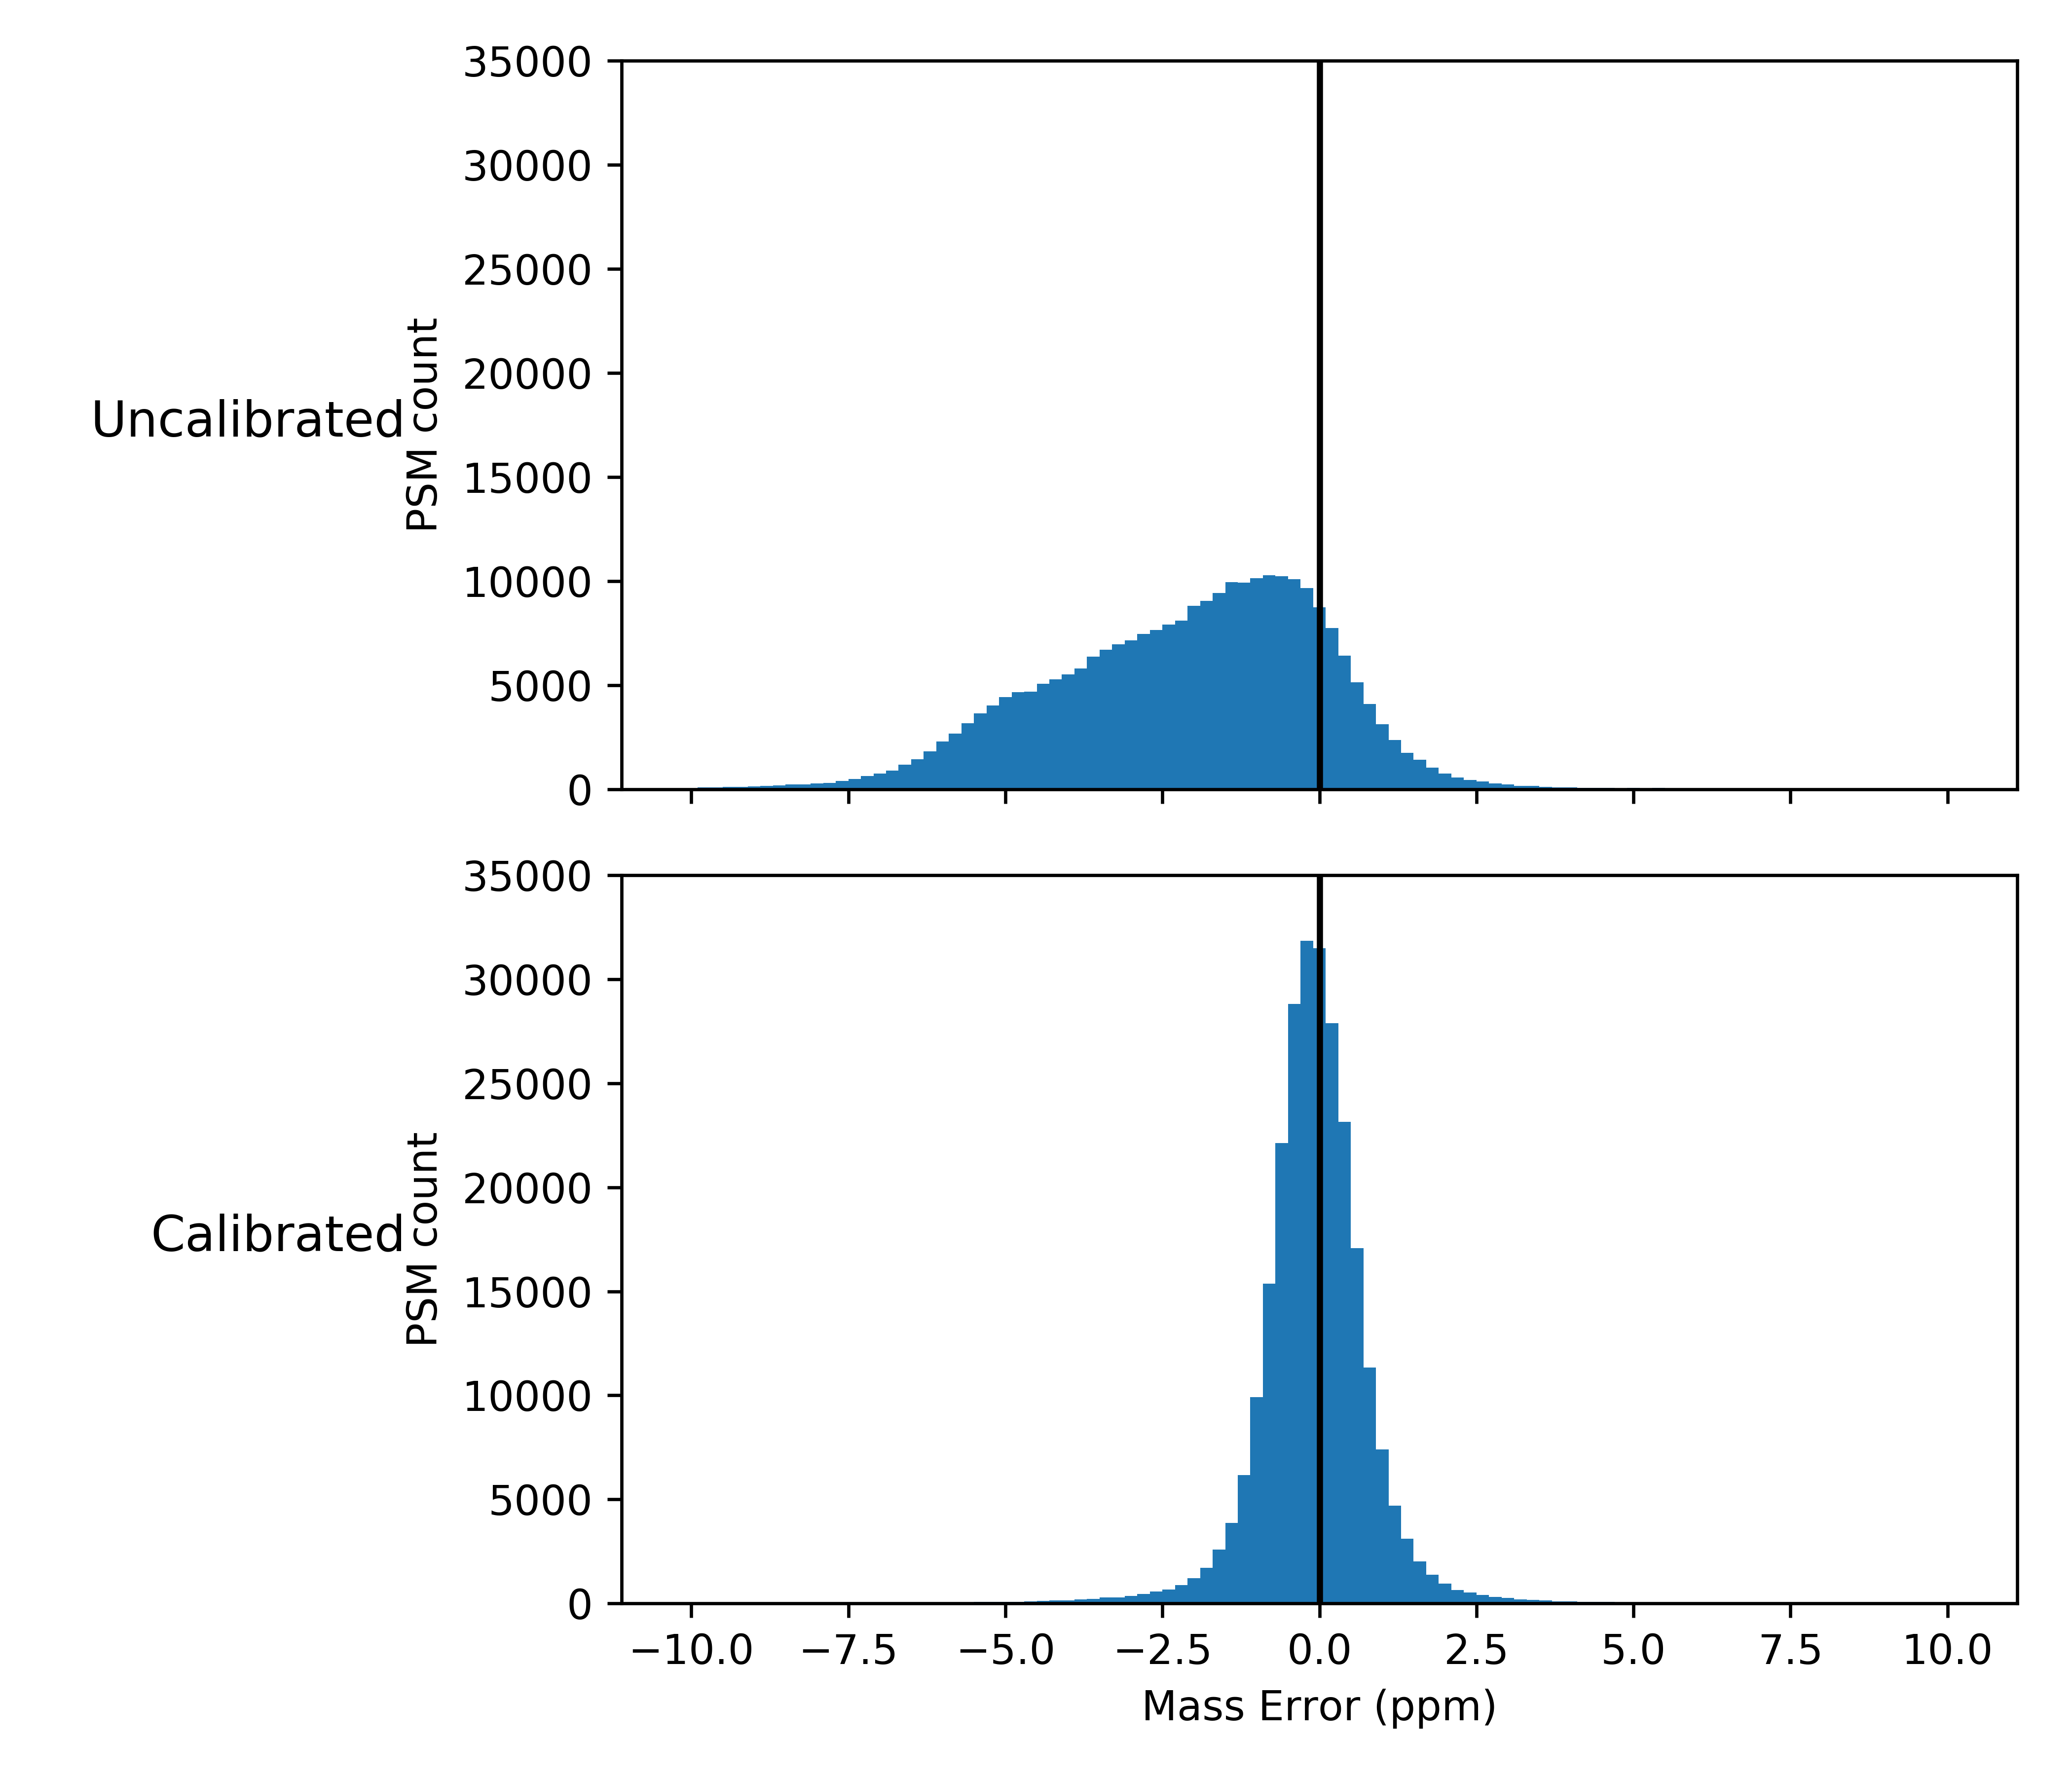
\includegraphics{fig2-10ppmSearchCalib.png}
 \caption{Histograms of the mass errors in identified peptides before and after calibration}
 \label{fgr:fig2-10ppmSearchCalib}
\end{figure}

\newpage

\subsection{Multi-Notch Searches}

It is useful to carefully describe the two commonly used database search approaches, prior to defining multi-notch searches and the impact that they have on G-PTM-D performance.
A traditional narrow-window search in bottom-up proteomics considers potential matches between theoretical peptides and experimental spectra if the candidate peptide mass and the observed precursor mass are equal within some defined tolerance (e.g. 5ppm, or 2.1 Da).
The other common search is an open search (e.g. $\pm 500$ Da)\citep{Chick_2015,Kong_2017,Li_2016}.
In searches of that type, the precursor mass and the mass of the best matching theoretical peptide could be many Da apart.
We describe an alternative to these search modes: the \textit{multi-notch} search.
This search is an extension of the narrow-window search that allows a variety of multiple specific mass differences between precursor mass and theoretical mass (See Figure~\ref{fig:fig3-searchTypes}) where the mass difference is easily interpretable.
It can also be seen as a narrowing of the open search to only allow prespecified mass differences.
One example of multi-notch search is the \textit{limited multi-notch} search, with notches at masses corresponding to Dalton differences between the monoisotopic peak and other peaks in averagine\citep{Senko1995} isotopic envelopes (e.g. 1.0029, 2.0054).
The advantages and disadvantages of this alternative strategy are described below.

\begin{figure}[H]
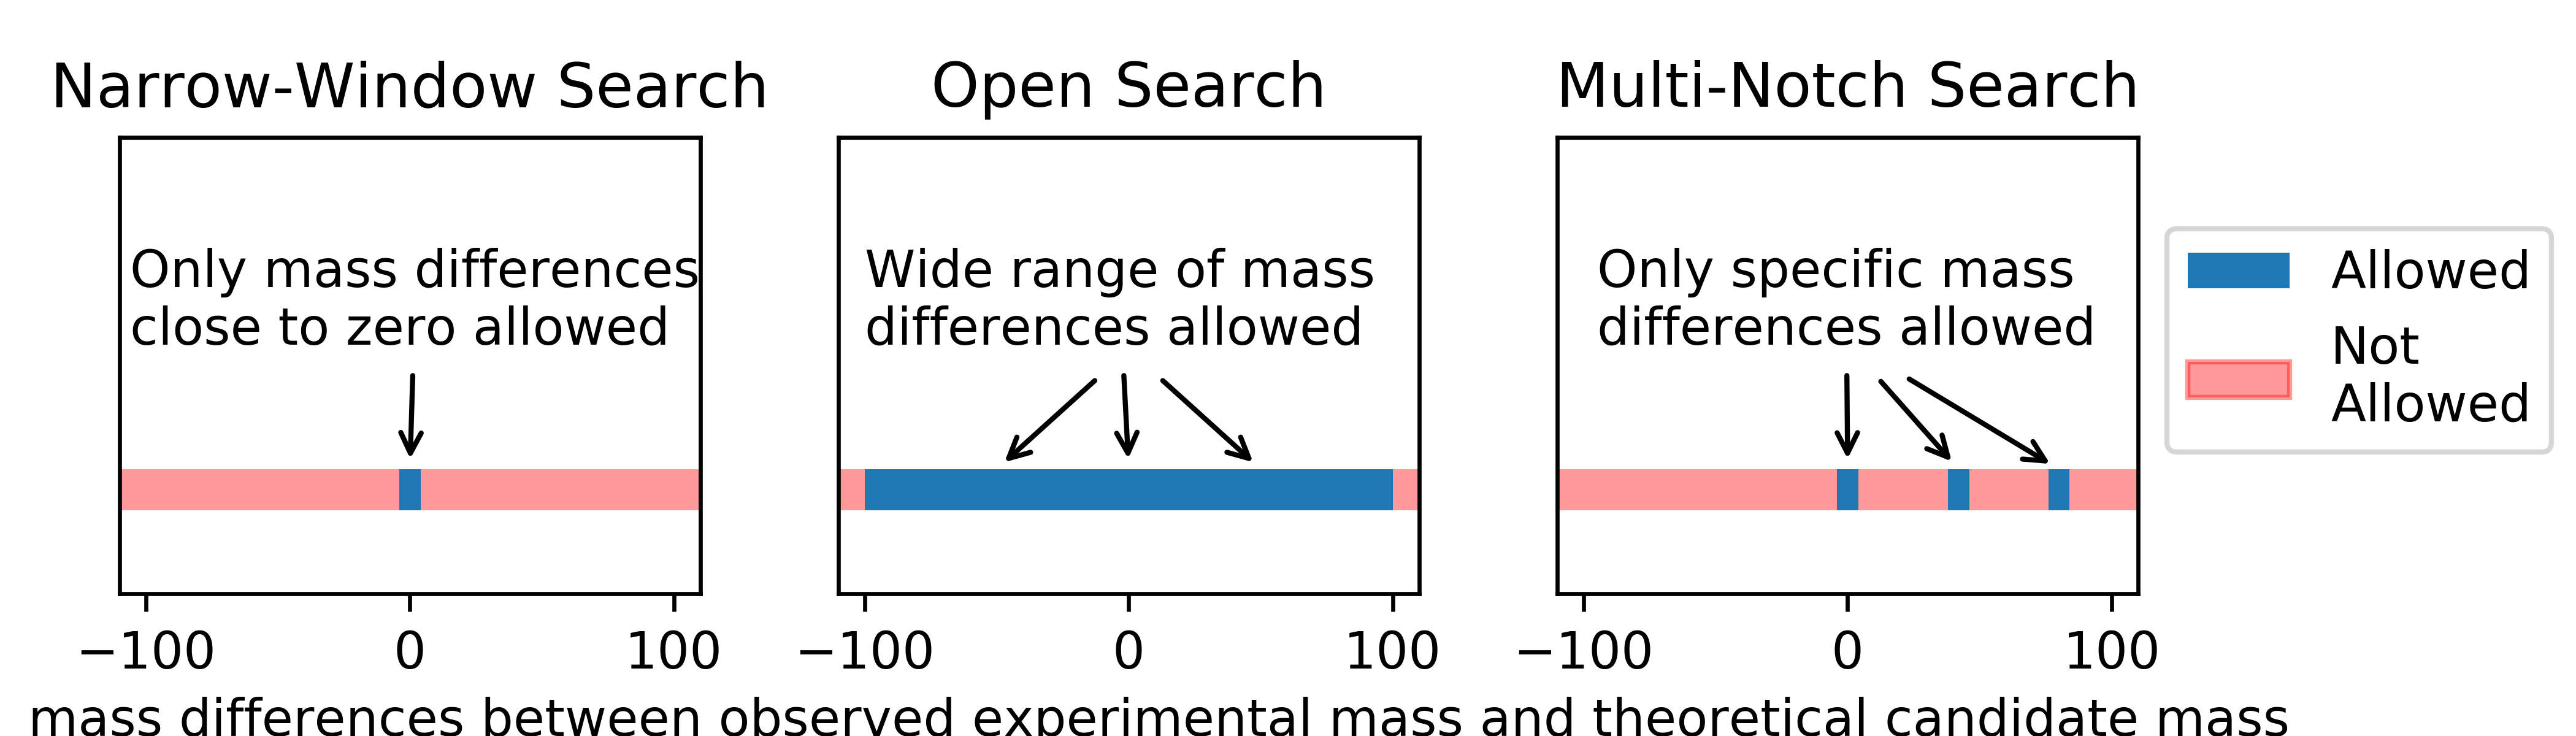
\includegraphics{fig3-searchTypes.png}
\caption{The three searches illustrated. Blue regions signify the allowed mass differences, while the pink ones show the mass differences that are not considered.}
\label{fig:fig3-searchTypes}
\end{figure}

\subsubsection{Traditional Narrow-Window Search vs. Limited Multi-Notch Search}

The traditional narrow-window search limits the range of acceptable mass differences between a candidate peptide and the observed experimental precursor in order to find an exact match to the observed peptide in a protein database.
A mass tolerance of <20ppm is commonly used on high-resolution MS1 data, resulting in a highly restrictive search.
It is not uncommon for the precursor mass tolerance of narrow-window searches to be relaxed to as much as 2 or 3 Da.
One rationale for this is that errors in the deisotoping of MS1 spectra frequently result in a reported experimental precursor mass being different by 1.0029 or 2.0054 Da from the true isolated peptide mass.
The relaxed tolerance approach identifies those peptides correctly.
A second rationale for this approach is that multiple peptides are frequently co-isolated and co-fragmented with all peptide fragments being observed in the same tandem mass spectrum.
Frequently, the best-fragmented peptide is different from the one corresponding to the precursor mass reported by the instrument, and the relaxed tolerance approach may identify this peptide, provided the reported charge state matches.
The major limitation of this approach is that a 2 or 3 Da tolerance includes mass differences that, when present, may indicate that the matched peptide is not the correct identification, arguably defeating the purpose of a narrow-window search.
This may happen when the mass difference arises due to the identified peptide being different from the actual isolated precursor by a low mass modification or amino acid substitutions.
The described issues are apparent in mass difference histograms in Figure~\ref{fig:fig4jurkat-1012}, generated by compiling the results of a 2.5 Da tolerance narrow-window search.
These plots clearly show that numerous peptides have missed monoisotopic peaks, deamidation, or an amino acid substitution.


\begin{figure}[H]
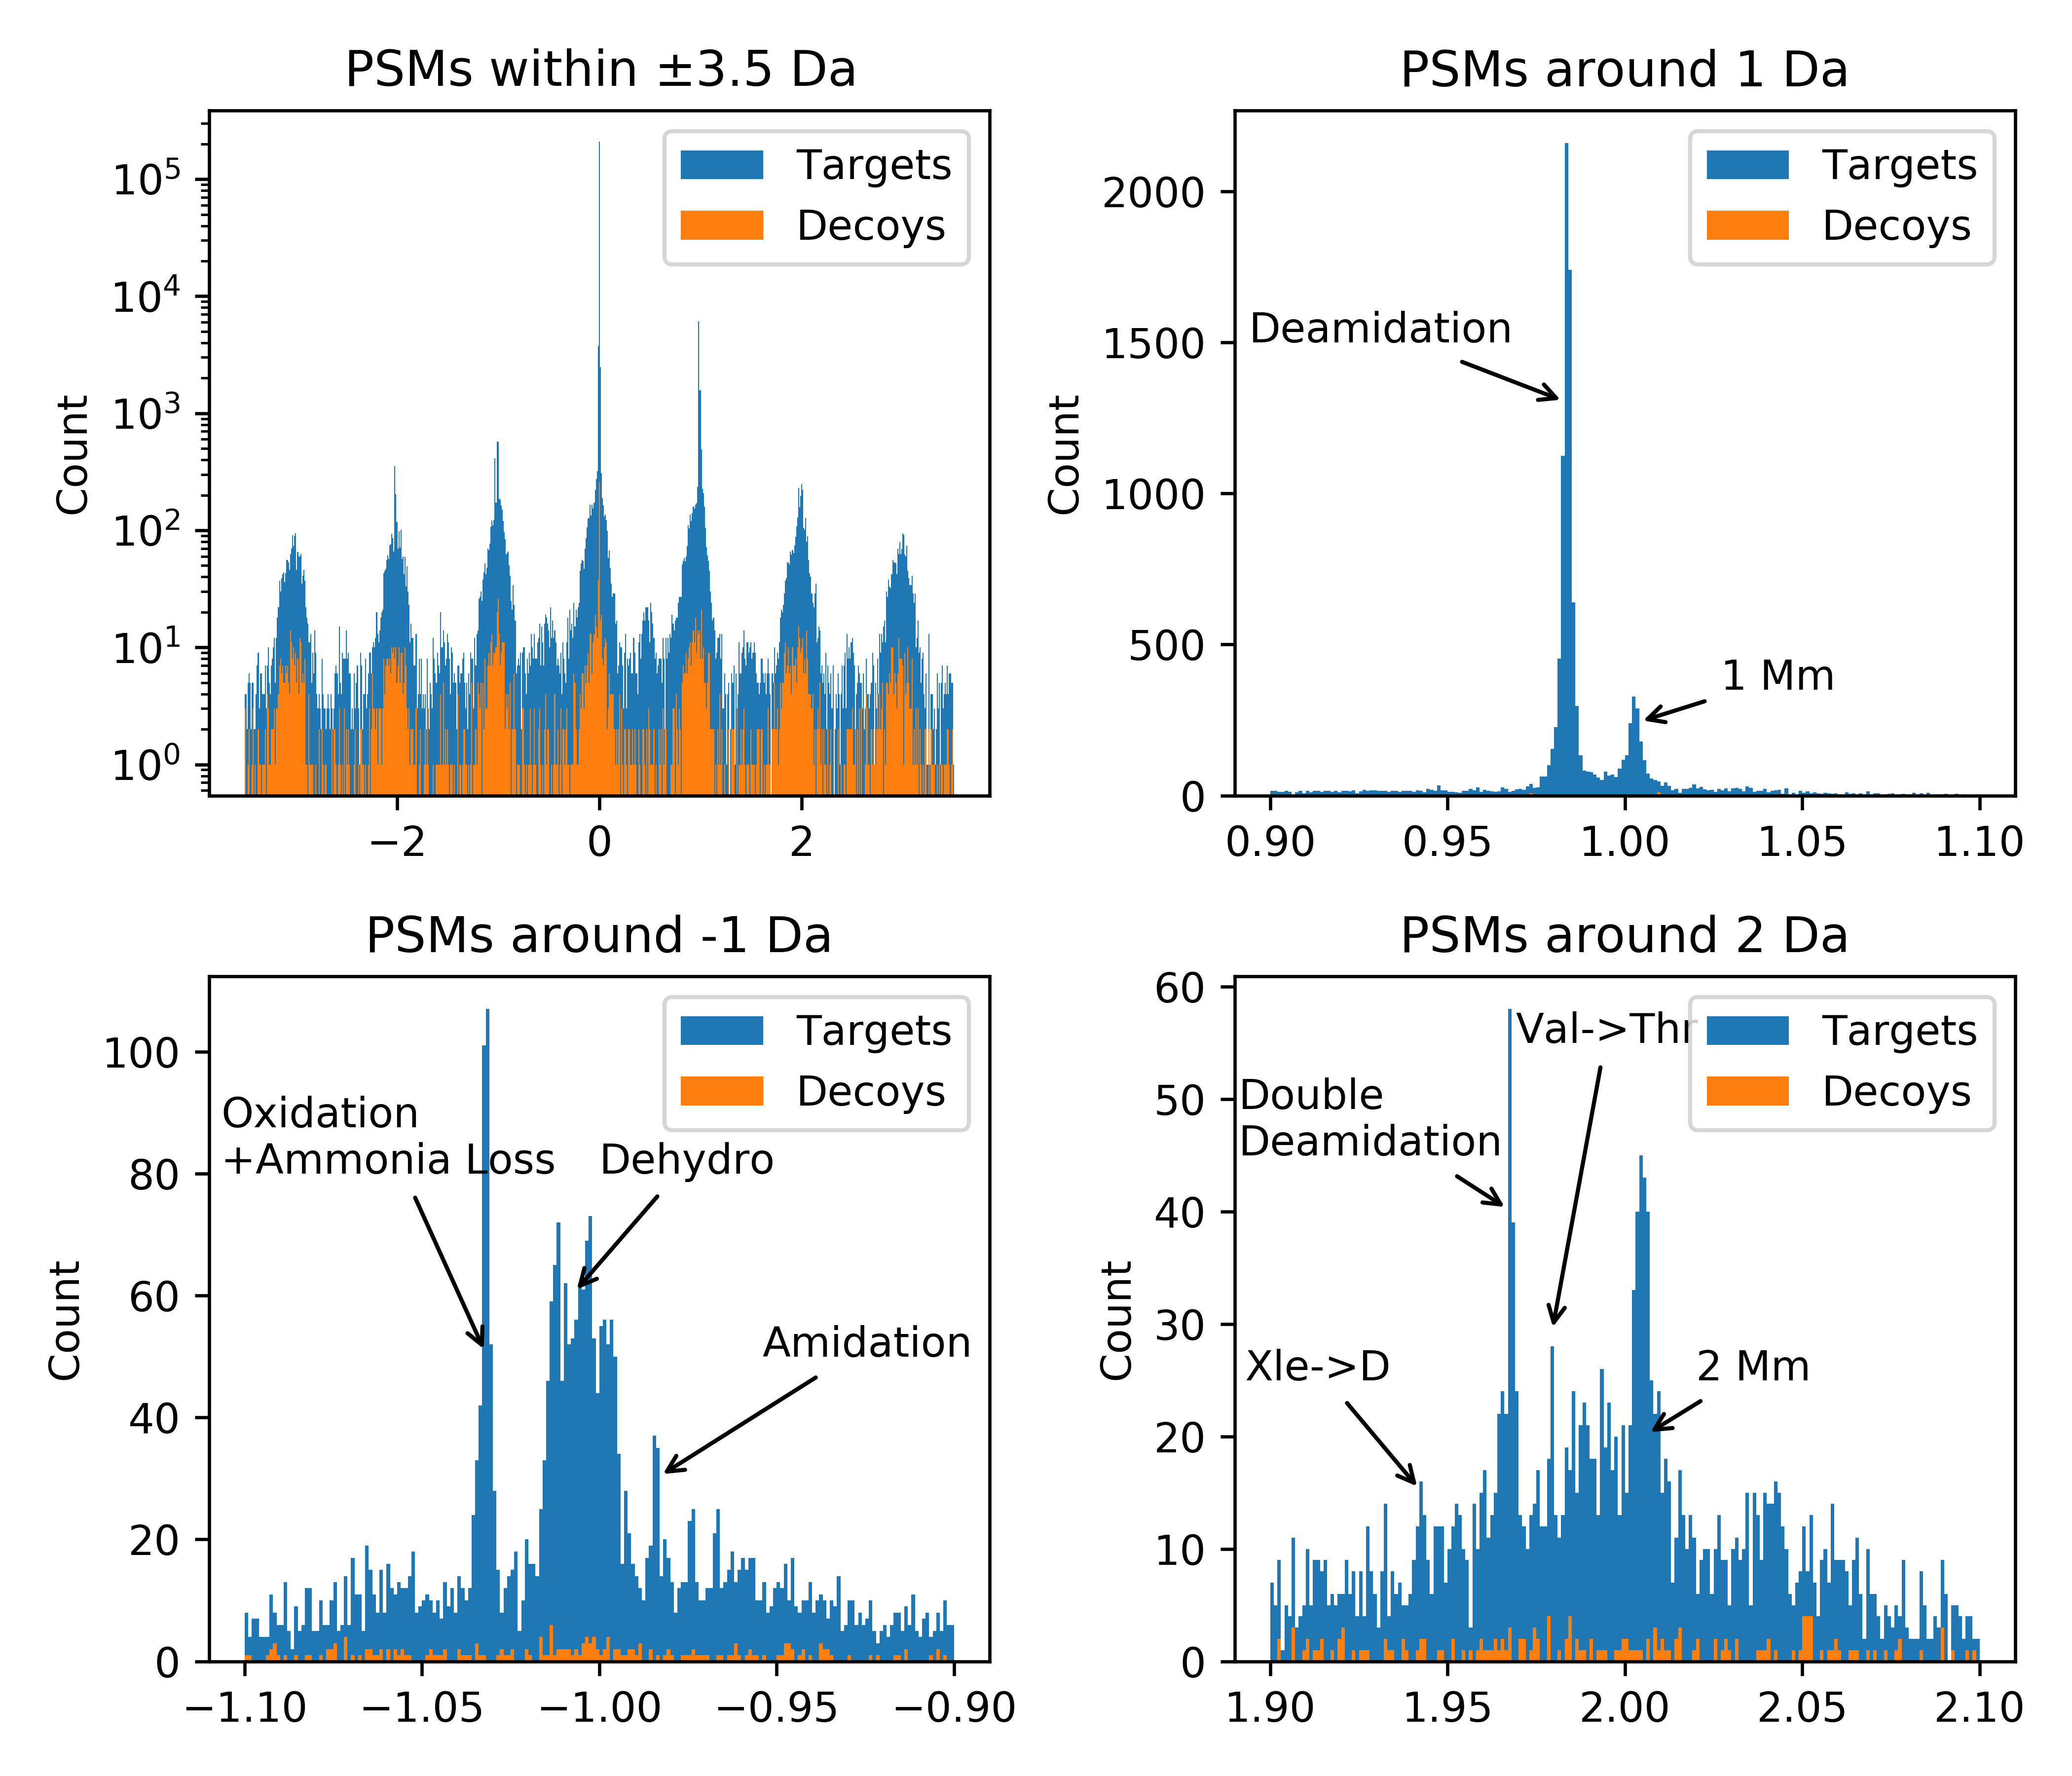
\includegraphics{fig4jurkat-1012.png}
\caption{Histograms of PSM mass differences found in various dalton ranges. MM, Missed Monoisotopic peak; Asp, Aspartic Acid; Asn, Asparagine; Glu, Glutamic Acid; Gln, Glutamine; Xle, Leucine/Isoleucine; Val, Valine; Thr, Threonine; Pro, Proline.}
\label{fig:fig4jurkat-1012}
\end{figure}

We propose a limited multi-notch search as a remedy to the trade-offs caused by choosing a narrow (few ppm) or wide (few Da) precursor mass tolerance during a traditional narrow-window search.
This limited multi-notch search allows mass differences between precursor and theoretical peptides of 0, 1.0029 and 2.0054 Da, but it limits the width around these three mass differences to a few ppm (e.g. 1-20 ppm).
This approach provides a means of getting an increased number of correct identifications while mitigating problems with incorrect identifications.
This alternative would appear to result in loss of identification of co-isolated peptides, but MetaMorpheus is programmed to handle this problem by identifying multiple co-isolated precursor masses (see section below).

To illustrate the described advantages, we compared the three types of searches using all 28 calibrated Jurkat fractions (Table~\ref{tbl:singleVsMultiNotch}).
The limited notch search yields the largest number of confidently identified PSMs with only a small fraction being misassigned.
We consider PSMs to be misassigned if the G-PTM-D procedure determines a higher-scoring modified peptide for a PSM (see the last section for details).
One example of a misassigned PSM, in the 2.5 Da Search, is the example where the correct identification has oxidation and ammonia loss, but was identified as an unmodified peptide with score 9.039 and mass difference of -1.0334 Da, with sequence \texttt{QAFDDAIAELDTLNEDSYK}, in Jurkat fraction 9 scan 20962.
With G-PTM-D added modifications, the correct peptide is identified with sequence \texttt{[Ammonia los]QAFDDAIAELDTLNEDSY[Oxidation]K}. It has a mass difference of -0.0017(-0.7946 ppm) and a score of 19.222.
While this kind of misassignment is not possible in the 5ppm narrow-window search, such missed monoisotopes are often assigned to a wrong sequence.
This explains the higher number of misassignments in the 5ppm search over the number in the multi-notch search.
Finally, even the multi-notch search has some misassignments.
One example, in Jurkat fraction 6 scan 15602, is the wrong identification of \texttt{SIQEIQELDK[acetyl]DDESLR} with a score of 10.153, when the correct identification, after the G-PTM-D procedure, is \texttt{S[acetyl]IQEIQELDKDDESLR} with score 16.249, where the masses are identical.
While all of the described searches have some misassigned false positive identifications, the multi-notch search minimizes them while also yielding the most PSMs.

\begin{table}[]
\centering
\caption{Multi-Notch Search vs Narrow-Window Search comparison of PSMs for Jurkat}
\label{tbl:singleVsMultiNotch}
\begin{tabular}{llll}
                    & 5ppm Search & 2.5 Da Search & Limited Multi-Notch Search \\
PSMs Within 1\% FDR & 275359      & 262543        & 279895       \\
Misassigned PSMs    & 2041           & 9041          & 1371            \\
\end{tabular}
\end{table}

\subsubsection{Multi-Notch Search vs. Open Search}

Chick et al. showed that by significantly relaxing the precursor mass tolerance in bottom-up searches, an incredible variety of unforeseen peptides were being fragmented and could be identified\citep{Chick_2015}.
In particular, PTM-containing peptides could be identified from MS2 fragments that did not possess the modification, and the type of PTM could be inferred from differences in identified peptide mass and precursor mass.
A major limitation of the Chick work was the extremely long search times because of the vast number of theoretical candidate peptides that were evaluated for each and every MS2 spectrum.
Recently, Kong\citep{Kong_2017} reported a new index-based search strategy (MSFragger) that radically improved search speeds for open searches.
$\pm 500$ Da precursor tolerance searches saw a 100-fold improvement in speed over most existing proteome database search tools.
The output of both search strategies is a list of PSMs, where the best matching unmodified theoretical peptide was found for each MS2 fragmentation spectrum and the mass difference between the theoretical and experimental precursor masses was determined.
The mass differences can be clustered into histogram peaks\citep{Rodriguez_2014}, with interpretation of the mass difference left as an exercise for the user.

There is a major problem with using the results from unrestricted precursor mass tolerance searches to infer peptide modifications regardless of whether they are of the Chick or Kong variety.
The freedom in precursor mass difference results in a multitude of false positive \textit{mass difference identifications}.
For example, small missed cleavages are often reported as mass differences.
The peptide \texttt{PEPKK} is often identified as \texttt{PEPK} with a mass error of 128 Da (the converse is also true, \texttt{PEPK} may be identified with a mass error of -128 Da).
Another example of this relates to peptide modifications.
The phosphopeptide \texttt{PEP[Phospho]SK} could be reported with a mass error of -79.96 Da when the better identification would have been \texttt{PEPSK}.
These simple errors are relatively easy to spot, but not when there are missed cleavages with multiple amino acids and/or multiple PTMs.

The alternative we recommend, is the use of a multi-notch search, which offers a means of reducing the search space and limiting the number of theoretical candidates to those plausible for the scan, increasing the search speed and most importantly, producing the most correct PSMs with the fewest false positive PSM identifications.
We compared searches of all Jurkat fractions using a $\pm 500$ Da wide mass search to a multi-notch search with notches at 0 and 79.961 with 0.02 Dalton tolerance.
The advantage of the multi-notch search over the open search is shown in Table~\ref{tbl:multiVsWide} by at least a $10\%$ increase in the number of target PSMs with score of at least 9.079, for both regions (0 Da no-PTM peptides and +79.96 Da phosphorylated and sulfonated peptides).
It is important to point out that the difference in the numbers of PSMs is not due to FDR considerations, but rather to erroneous peak assignments in open searches, that misassign PSMs due to the extreme freedom in precursor masses allowed in open searches.
A specific example of a PSM that has been erroneously assigned in a open search is scan 12835 in Jurkat fraction 5.
The open search identifies \texttt{ATPARAPESPPSADPALVAGPAEEAEC[Carbamidomethyl]PPPR} as the best match with a score of 17.231 and mass difference of -416.3103, and a single missed cleavage.
The better match is identified by the multi-notch search, as \texttt{APESPPSADPALVAGPAEEAEC[Carbamidomethyl]PPPR} with a score of 16.246 and mass difference of 79.9655, and no missed cleavages.
So, instead of having a PSM with an unidentifiable mass difference of -416.3103 (mass of removal of \texttt{ATPAR} and addition of phosphorylation), we have an easily identifiable mass difference corresponding to a phosphorylation site.

\begin{table}[]
\centering
\caption{Number of PSMs in Multi-Notch Search vs. Open Search for select mass differences.}
\label{tbl:multiVsWide}
\begin{tabular}{lll}
               & Open                     & Multi-Notch         \\
0 peak         & 176073  (0.15\% FDR)     & 193328 (0.23\% FDR) \\
79.96 peak     & 732   (0.68\% FDR)       & 957  (0.84\% FDR)   \\
\end{tabular}
\end{table}

\subsection{Co-isolation}

Peptide co-isolation and co-fragmentation complicates mass spec data analysis, but carefully taking co-isolation into account provides substantially better results~\cite{Zhang2014}.

Consider the Jurkat fraction 12 scan 12336 with precursor scan 12333.
Isolation m/z is 726.65 Th and isolation width is 2.5 Th.
It is shown in Figure~\ref{fig:fig5-coIsolationSpectrum}.
There are at least three different peptides being co-isolated and co-fragmented, and there is evidence in the MS/MS spectrum for all of them.

\begin{figure}[H]
\includegraphics{fig5-coIsolationSpectrum.png}
\caption{m/z peaks in MS1 scan 12333. The top plot shows the isotopic envelopes for three distinct peptides in a narrow isolation window. The bottom plot shows some identified fragment peaks in the MS/MS scan.}
\label{fig:fig5-coIsolationSpectrum}
\end{figure}

In a conventional search, only the isolation m/z value of 726.65 would be used to select a range of theoretical peptides for comparison.
Assuming correct de-isotoping and charge state calculation, the mass 1447.74 Da would be searched.
However, all peptides in the range 725.4 to 727.9 Th are co-fragmented and a better solution would be to use all co-isolated precursor masses.
In MetaMorpheus, for each MS2 scan, the corresponding MS1 scan is deconvoluted and the complete list of precursors is gathered for the range surrounding the isolated precursor ($\pm 1.25$ Th).
Each deconvoluted mass is used to select a range of theoreticals to use for identification.
The result of this is that often, more than one peptide can be identified from a single MS2 scan.
This is extremely beneficial in both open mass and multi-notch searches because it reduces the number of the more difficult to interpret mass differences and substantially improves G-PTM-D (see below).

\subsection{Enhanced G-PTM-D Results}

In the original G-PTM-D manuscript\citep{Li_2016}, an open mass search ($\pm 200$ Da) was used to create a histogram of mass difference peaks, from which PTMs could be inferred.
A Perl script was used to mine those mass differences to modify a proteomics database with potential PTMs.
This database was used for a final search and numerous PTMs were identified.
While that work represented a substantial conceptual advance in identifying PTMs, there were several limitations to its utility.
One, the open mass search was unacceptably slow.
Two, uncalibrated data made it hard to discern closely spaced modifications.
Three, certain mass differences with high FDRs were incorrectly allowed.
Four, missed monoisotopic peaks and co-isolated peaks were not handled.
Five, separate programs were required (both Morpheus and a Perl script).
Six, the small list of 13 PTMs did not include many important modifications.
MetaMorpheus resolves all of these issues and more.
In the preceding sections, we detailed the performance improvements introduced by each enhancement: in this section we show their combined effect.
Every comparison is a contrast of results from the original G-PTM-D workflow with the fully enhanced one.

A major improvement in G-PTM-D performance arises from using calibrated spectra as inputs to the procedure.
Calibration and the associated increase in mass accuracy is essential for discrimination of small differences between mass differences due to different modifications.
To illustrate this, mass differences around 80 Daltons from the initial notch search are aggregated in the histograms in Figure~\ref{fig:fig7-PhosphoAndSulfo}.
It is evident from these histograms that the phosphorylation and sulfonation peaks are clearly separated and identifiable when the search is conducted on well-calibrated spectra.


\begin{figure}[H]
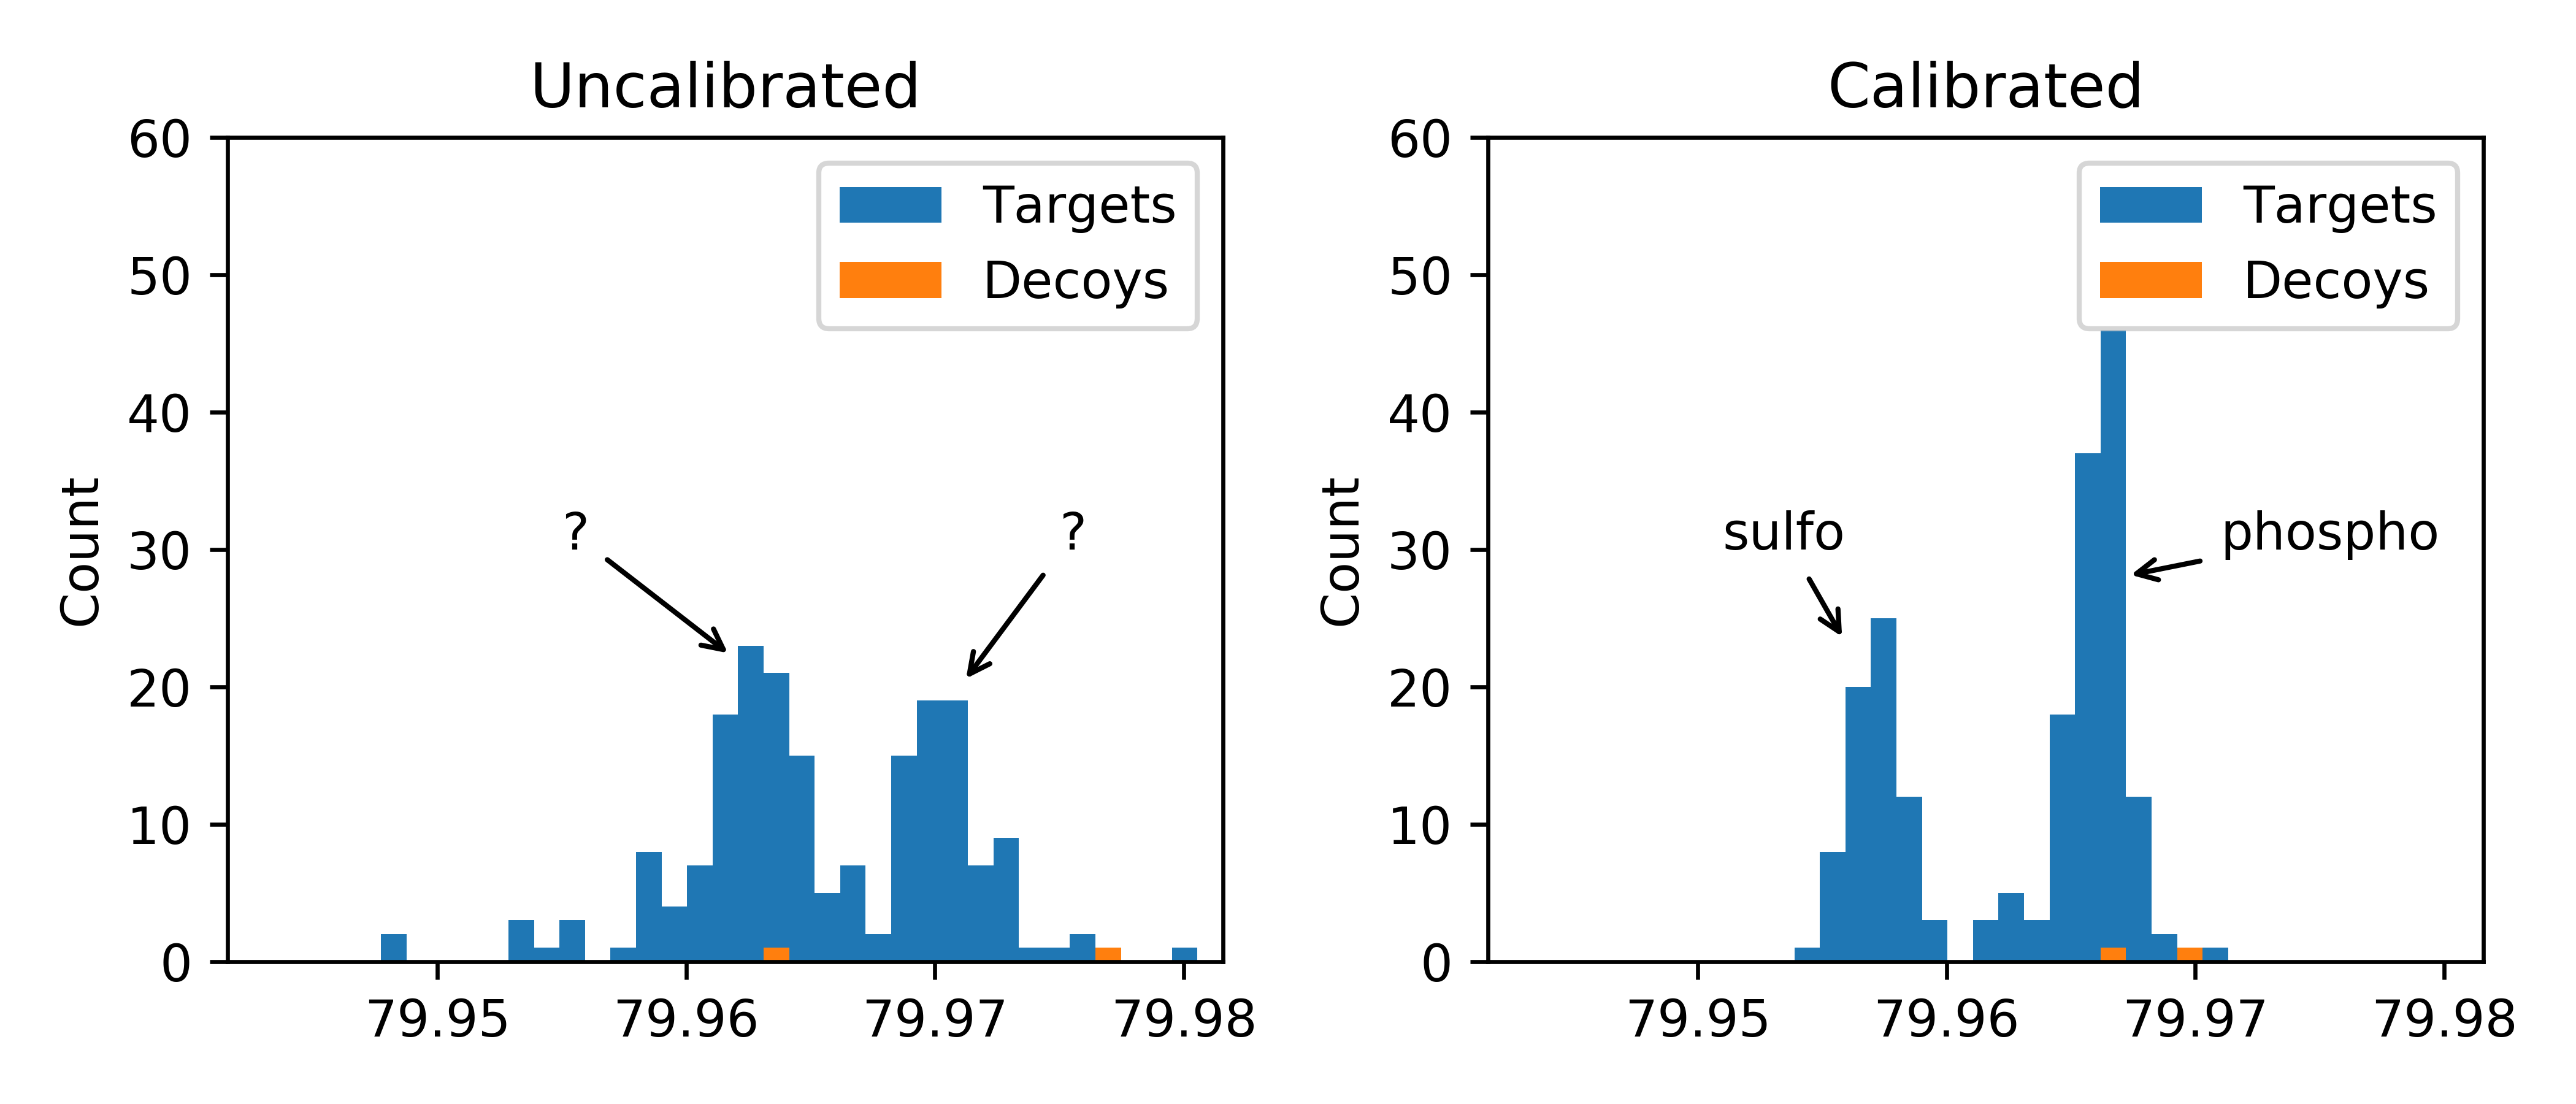
\includegraphics{fig7-SulfoAndPhospho.png}
\caption{Peaks around phosphorylation and sulfonation in uncalibrated and calibrated data}
\label{fig:fig7-PhosphoAndSulfo}
\end{figure}

The next step, database augmentation, outputs significantly different augmented databases because of the difference between accepted mass differences in the open and the multi-notch searches.
At this point, another advantage of the enhanced approach is clear; the overall search time dropped significantly, from 35 hours to 4 hours for all datasets (see Table~\ref{my-labelff}).

\begin{table}[]
\centering
\caption{Effects of Replacing Initial Open Search by a Multi-Notch Search}
\label{my-labelff}
\begin{tabular}{llll}
                      &        & Open Search & Multi-Notch Search\\
\multirow{2}{*}{Time} & Jurkat & 22.1 hrs         & 2.9 hrs    \\
                      & Mouse  & 13.5 hrs         & 1.2 hrs   \\
\end{tabular}
\end{table}

After the final search using the augmented database is conducted (narrow-window in the original, and limited multi-notch in the enhanced G-PTM-D), the numbers of PSMs, peptides, and proteins all increase as shown in Table~\ref{tab:table2}.
We identified hundreds of glycosylated peptides in these unenriched samples, with many of these modifications exceeding 1000 Da, see Table~\ref{tab:table3}.
These enhancements demonstrate that the enhanced G-PTM-D approach provides great value to bottom-up proteomic data analysis.
It is fast enough included as part of every regular work-flow, and will yield significantly increased numbers of correctly identified PTM peptides.

\begin{table}[]
\centering
\caption{Enhanced G-PTM-D overall improvement numbers}
\label{tab:table2}
\begin{tabular}{llll}
                      &        & Original G-PTM-D & Enhanced G-PTM-D\\
\multirow{2}{*}{PSMs} & Jurkat  & 210566   &  220574  \\
                      & Mouse    & 162473   &   170743 \\
\multirow{2}{*}{Unique Peptides} & Jurkat  & 85542   &  101980  \\
                      & Mouse    & 56235   &   66365 \\
\multirow{2}{*}{Proteins} & Jurkat  & 9254   &  9587  \\
                      & Mouse    & 7874   &   8151 \\
\multirow{2}{*}{PTM containing peptides} & Jurkat  & 12041   &  22173  \\
                      & Mouse    & 14547   &   18487 \\
\end{tabular}
\end{table}


\begin{table}[]
\centering
\caption{Highest mass PTMs identified}
\label{tab:table3}
\begin{tabular}{ll}
Mass (Daltons)&	Mod\\
1378.474&	Hex(6)HexNAc(2)\\
1216.4236&	Hex(5)HexNAc(2)\\
1054.3719&	Hex(4)HexNAc(2)\\
1038.375&	dHex(1)Hex(3)HexNAc(2)\\
963.3177&	Hex(1)HexNAc(1)NeuAc(1)NeuGc(1)
\end{tabular}
\end{table}


%\begin{acknowledgement}

%The authors thank \ldots
%\end{acknowledgement}

%\begin{suppinfo}

%The following files are available free of charge.
%\begin{itemize}
%  \item Filename: brief description
%  \item Filename: brief description
%\end{itemize}

%\end{suppinfo}

\bibliography{citations}

\end{document}
